% !TEX root = ../MasterThesis_Onoe.tex
% 上記はただのコメントではなく親ファイルの場所を教えているので
% 消してしまうとファイルごとのタイプセットができなくなるので注意。
% 親ファイル名を変更したときはここも変更する。

\externaldocument{Deeplearning}

\chapter{深層学習を用いたジェットフレーバー識別} \label{sec:Flavortagging}
本章では、深層学習を用いて開発したジェットフレーバー識別アルゴリズムについて述べる。まず5.1節では、フレーバー識別に関係する事象の詳細についてや、現在ジェットフレーバー識別に用いられているLCFIPlusについて述べる。次に3.2節で、今回のアルゴリズムの評価において使用したMCシミュレーションデータについて述べる。またシミュレーションデータには深層学習における精度を上げるために前処理を行なっており、これについても述べる。そして5.3節、5.4節それぞれでディープニューラルネットワーク、グラフニューラルネットワークによる実装について述べ、5.5節でLCFIPlusと比較を行って学習の性能について議論する。
\section{ジェットフレーバー識別アルゴリズム}
\subsection{事象について}

\subsection{LCFIPlusにおけるフレーバー識別}
LCFIPlusのフレームワークでは、フレーバー識別は崩壊点検出、ジェットクラスタリングの後に行われる。フレーバー識別は、飛跡や崩壊点の特徴量をもとにROOTのTMVAパッケージにおけるBoosted Decision Trees (BDTs) を用いて識別が行われる。このBoosted Decision Treesは、複数のモデルを組み合わせて全体的な性能を向上させるアンサンブル学習 (Boosting) と、入力された特徴量に基づいてデータをクラスに分割していく決定木 (Decision Tree) の手法を組み合わせたものであり、複数の弱い決定木モデルを組み合わせて決定木の精度を向上させる機械学習手法である。データは、初めに崩壊点の数で場合分けが行われ、表\ref{lcfiplusin}にある入力変数をもとに、最終的に各ジェットをb/c/udsの3つに分類する学習を行う。
\begin{table}[H]
 \centering
 \small
  \begin{tabular}{ l | l }
   \hline
   変数名 & 説明\\
   \hline \hline
   nvtx & 崩壊点の数\\
   trk1d0sig & $d_0$のsignificanceが最も高い飛跡の$d_0$\\
   trk2d0sig & $d_0$のsignificanceが2番目に高い飛跡の$d_0$\\
   trk1z0sig & $z_0$のsignificanceが最も高い飛跡の$d_0$\\
   trk2z0sig & $z_0$のsignificanceが2番目に高い飛跡の$d_0$\\
   trk1pt & $d_0$が最も大きい軌道の横方向運動量\\
   tkr2pt & $d_0$が2番目に大きい軌道の横方向運動量\\
   jprobr & 全飛跡を用いたr-$\phi$平面での結合確率\\
   jprobr5sigma & 5$\sigma$以上のパラメータを持つ全飛跡を用いたr-$\phi$平面での結合確率\\
   jprobz & 全軌跡を用いたz軸射影での結合確率\\
   jprobz5sigma & 5$\sigma$以上のパラメータを持つ全飛跡を用いたz軸射影での結合確率\\
   d0bprob & 全飛跡に対してb,c,udsフレーバーの$d_0$分布を用いた$d_0$のb-クォーク確率の積\\
   d0cprob & 全飛跡に対してb,c,udsフレーバーの$d_0$分布を用いた$d_0$のc-クォーク確率の積\\
   d0qprob & 全飛跡に対してb,c,udsフレーバーの$d_0$分布を用いた$d_0$のuds-クォーク確率の積\\
   z0bprob & 全飛跡に対してb,c,udsフレーバーの$z_0$分布を用いた$d_0$のb-クォーク確率の積\\
   z0cprob & 全飛跡に対してb,c,udsフレーバーの$z_0$分布を用いた$d_0$のc-クォーク確率の積\\
   z0qprob & 全飛跡に対してb,c,udsフレーバーの$z_0$分布を用いた$d_0$のuds-クォーク確率の積\\
   nmuon & ミューオンの数\\
   nelectron & 電子の数\\
   trkmass & $d_0/z_0$が5$\sigma$を超える全飛跡の質量\\
   1vtxprob & 崩壊点に関連した全飛跡を結合した時の崩壊点確率\\
   vtxlen1 & ジェット内の初めの崩壊点の崩壊長\\
   vtxlen2 & ジェット内の2番目の崩壊点の崩壊長\\
   vtxlen12 & ジェット内の初めの崩壊点と2番目の崩壊点の距離\\
   vtxsig1 & vtxlen1のsignificance\\
   vtxsig2 & vtxlen2のsignificance\\
   vtxsig12 & vtxlen12を初めの崩壊点と2番目の崩壊点の共分散行列の和の誤差で割った値\\
   vtxdirang1 & 運動量と初めの崩壊点の変位との間の開き角\\
   vtxdirang2 & 運動量と2番目の崩壊点の変位との間の開き角\\
   vtxmult1 & 初めの崩壊点に含まれる飛跡数\\
   vtxmult2 & 2番目の崩壊点に含まれる飛跡数\\
   vtxmult & secondary vertexを構成するために用いられる飛跡の数\\
   vtxmom1 & 初めのの頂点に結合された全飛跡の運動量のベクトル和\\
   vtxmom2 & 2番目の頂点に結合された全飛跡の運動量のベクトル和\\
   vtxmass1 & 飛跡の四元運動量の和から計算される初めの崩壊点質量\\
   vtxmass2 & 飛跡の四元運動量の和から計算される2番目の崩壊点質量\\
   vtxmass & secondary vertexを構成する全 飛跡の四元運動量の和から計算される崩壊点質量\\
   vtxmasspc & primary/secondary vertexの誤差行列で許容可能なpt補正を行なった崩壊点質量\\
   vtxprob & 崩壊点が形成される確率\\
   \hline
  \end{tabular}
  \caption{LCFIPlusにおけるフレーバー識別の入力変数}
 \label{lcfiplusin}
\end{table}
\section{イベントサンプル}
本研究では、MCイベントジェネレーターであるwhizardによる事象生成を行い、ILD検出器のフルシミュレーションを使用したデータを用いてフレーバー識別を行った。シミュレーションデータについての詳細を表\ref{data}に示す。
\begin{table}[H]
 \centering
 \begin{tabular}{ c c }
 \hline
 イベントジェネレーター & whizard\\
 検出器シミュレーション & ILD Full simulation\\
 反応過程 & $e^+e^- \rightarrow \nu \bar{\nu} h$\\
 重心系エネルギー & 250GeV\\
 ISR & なし\\
 ビーム偏極 & なし\\
 \hline
 \end{tabular}
 \label{data}
 \caption{シミュレーションデータの性質}
\end{table}
\section{ディープニューラルネットワークによる実装}
本節では、ディープニューラルネットワーク (多層ニューラルネットワーク) によるフレーバー識別の実装について述べる。
\subsection{実装目的}
フレーバー識別では、シグナル効率に対して排除できる背景事象の割合が多くなるほど、ヒッグスなどの物理解析において有利であるため、その性能が非常に重要である。LCFIPlusにおいて実装されているBDTsは、崩壊点やジェットの特徴量の場合分けによって分類を行うため、ツリー構造が視覚化されており解釈が容易である。一方で、BDTsの場合分けにおける閾値は人の手で定める必要があり、ILCのフレーバー識別のようなデータが高次元で複雑なタスクに対しては、より複雑な表現学習の方が適している可能性がある。さらにBDTsにはノイズに敏感である点や、ツリー数が多くなると過学習を起こす点など問題点もある。そこで本研究では、フレーバー識別の更なる性能向上を目的にディープニューラルネットワークによる実装を行った。ディープニューラルネットワークでは、データから複雑な表現を自動的に学習することができる。そのため、より最適化したモデルの獲得を目指すため、ディープニューラルネットワークでの実装を行った。
\subsection{入力変数とネットワークアーキテクチャ}
学習の入力変数は、LCFIPlusにおいて用いた変数 (表\ref{dnnin}) と同様の変数を使用した。また、学習値に対しては前処理を行い、0付近の値が多い変数や値幅が大きい変数が存在したため、各変数に対して対数変換や正規化を実行した。また出力もLCFIPlusと同様にbフレーバー、cフレーバー、udsフレーバーとした。\\
ネットワークには図\ref{dnnmodel}のように最も単純な全結合層を用いたニューラルネットワークを採用した。さらに、過学習を抑制するためにバッチ正規化を各全結合層の後に行い、活性化関数には勾配消失への対策として全てLeakyReLU関数を使用した。損失関数には分類問題に適した交差エントロピーを用い、最適化アルゴリズムにはAdamを学習率0.01で使用した。また学習率は25 epoch(学習データでの学習回数)ごとに0.1倍させ、学習の安定化を目的に学習率を減衰させた。表\ref{dnnsetting}に学習におけるハイパーパラメータをまとめる。
\begin{figure}[H]
	\begin{center}
 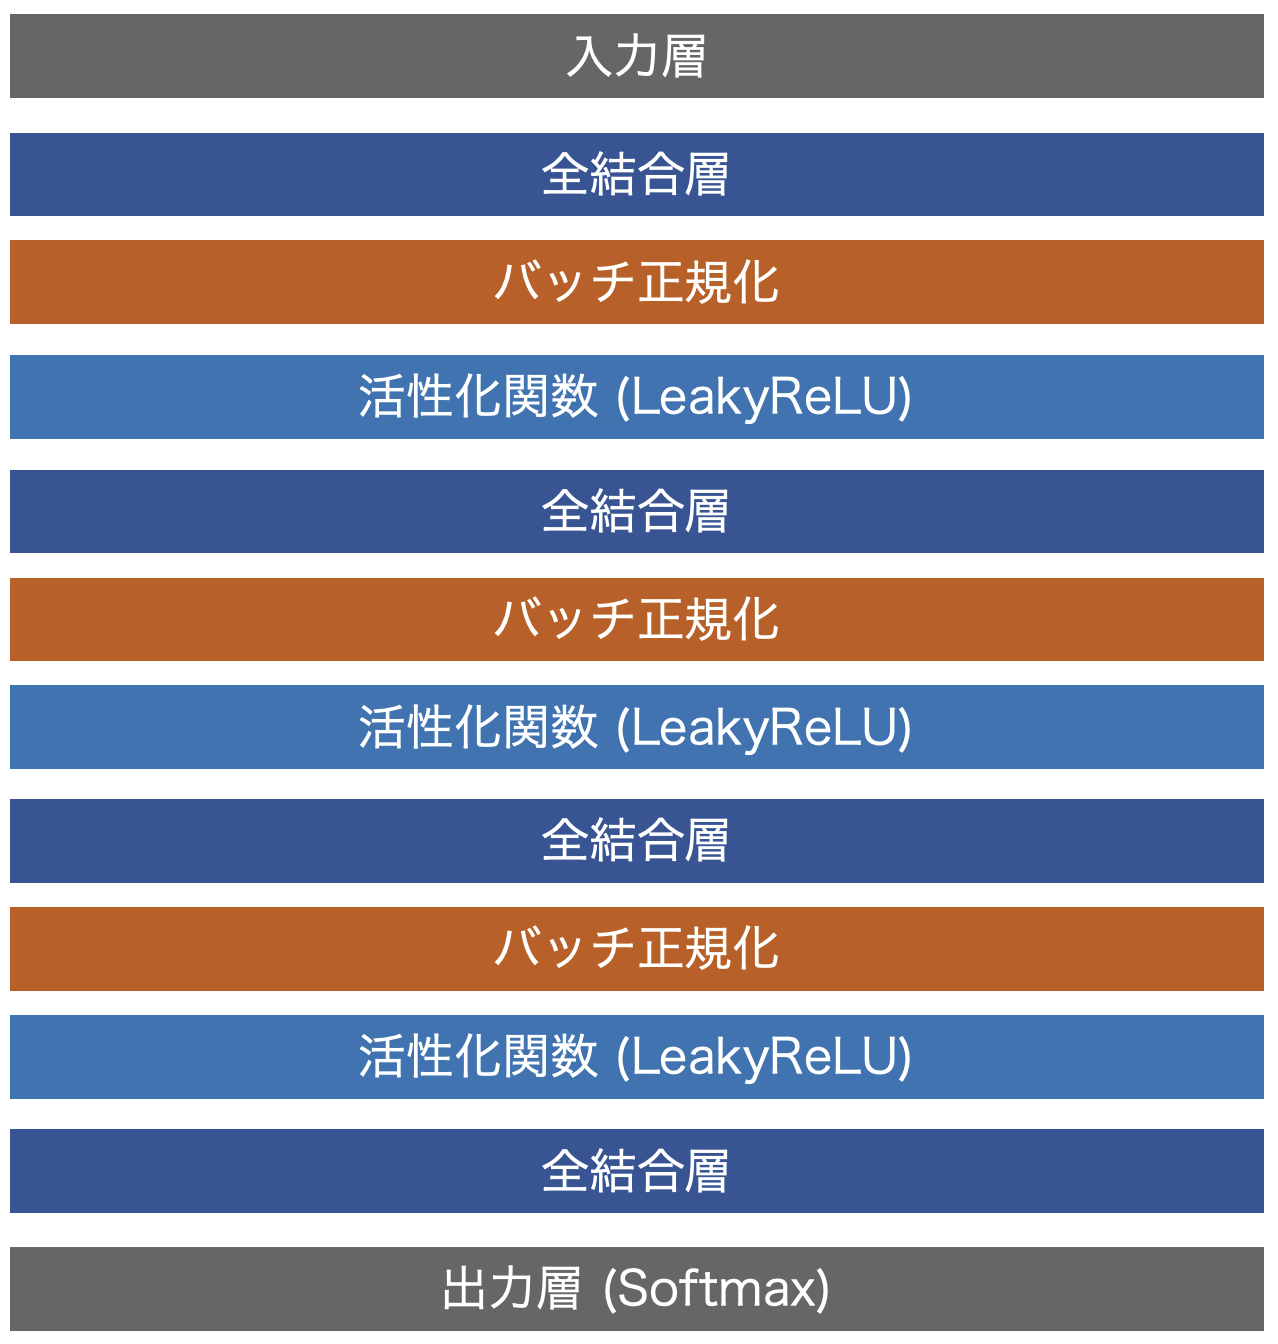
\includegraphics[keepaspectratio, scale=0.5]
 	{Figure/Flavortagging/dnn.png}
 		\caption{フレーバー識別のためのディープニューラルネットワークの概略図}
 		\label{dnnmodel}
	\end{center}
\end{figure}
\begin{table}[H]
 \centering
  \begin{tabular}{ l  l }
   \hline
   ノード数 & (124, 124, 124)\\
   活性化関数 & ReLU関数\\
   損失関数 & 交差エントロピー\\
   最適化アルゴリズム & Adam\\
   学習率 & 0.01 (25epochあたり0.1倍)\\
   エポック数 & 100\\
   バッチサイズ & 1024\\
   \hline
  \end{tabular}
  \caption{ディープニューラルネットワークにおけるハイパーパラメータ}
  \label{dnnsetting}
\end{table}
\subsection{ハイパーパラメータの最適化}
記入予定
\subsection{学習評価}
学習における損失関数の値と識別精度を図\ref{dnnoutput}に示す。100epochの学習によって、損失関数の値は降下したのちおおよそ安定しており、学習精度はおよそ$82.5\%$となっている。また、図\ref{dnncm}に混合行列を示す。混合行列とは、分類問題で出力された結果をまとめた表であり、縦軸 (行) が実際の答えを横軸 (列) が学習結果を表していて、実際の答えごと (行) に正規化されている。そのため、左上から右下の対角成分が実際の答えと学習結果が一致している割合を表しており、図\ref{dnnoutput}における学習精度は$(学習精度) = (対角成分の和) / (全成分の和)$として求められる。図\ref{dnncm}より、ディープニューラルネットワークではcジェットについてはudsジェットと識別しにくいことがわかる。\\
\begin{figure}[H]
	\begin{center}
 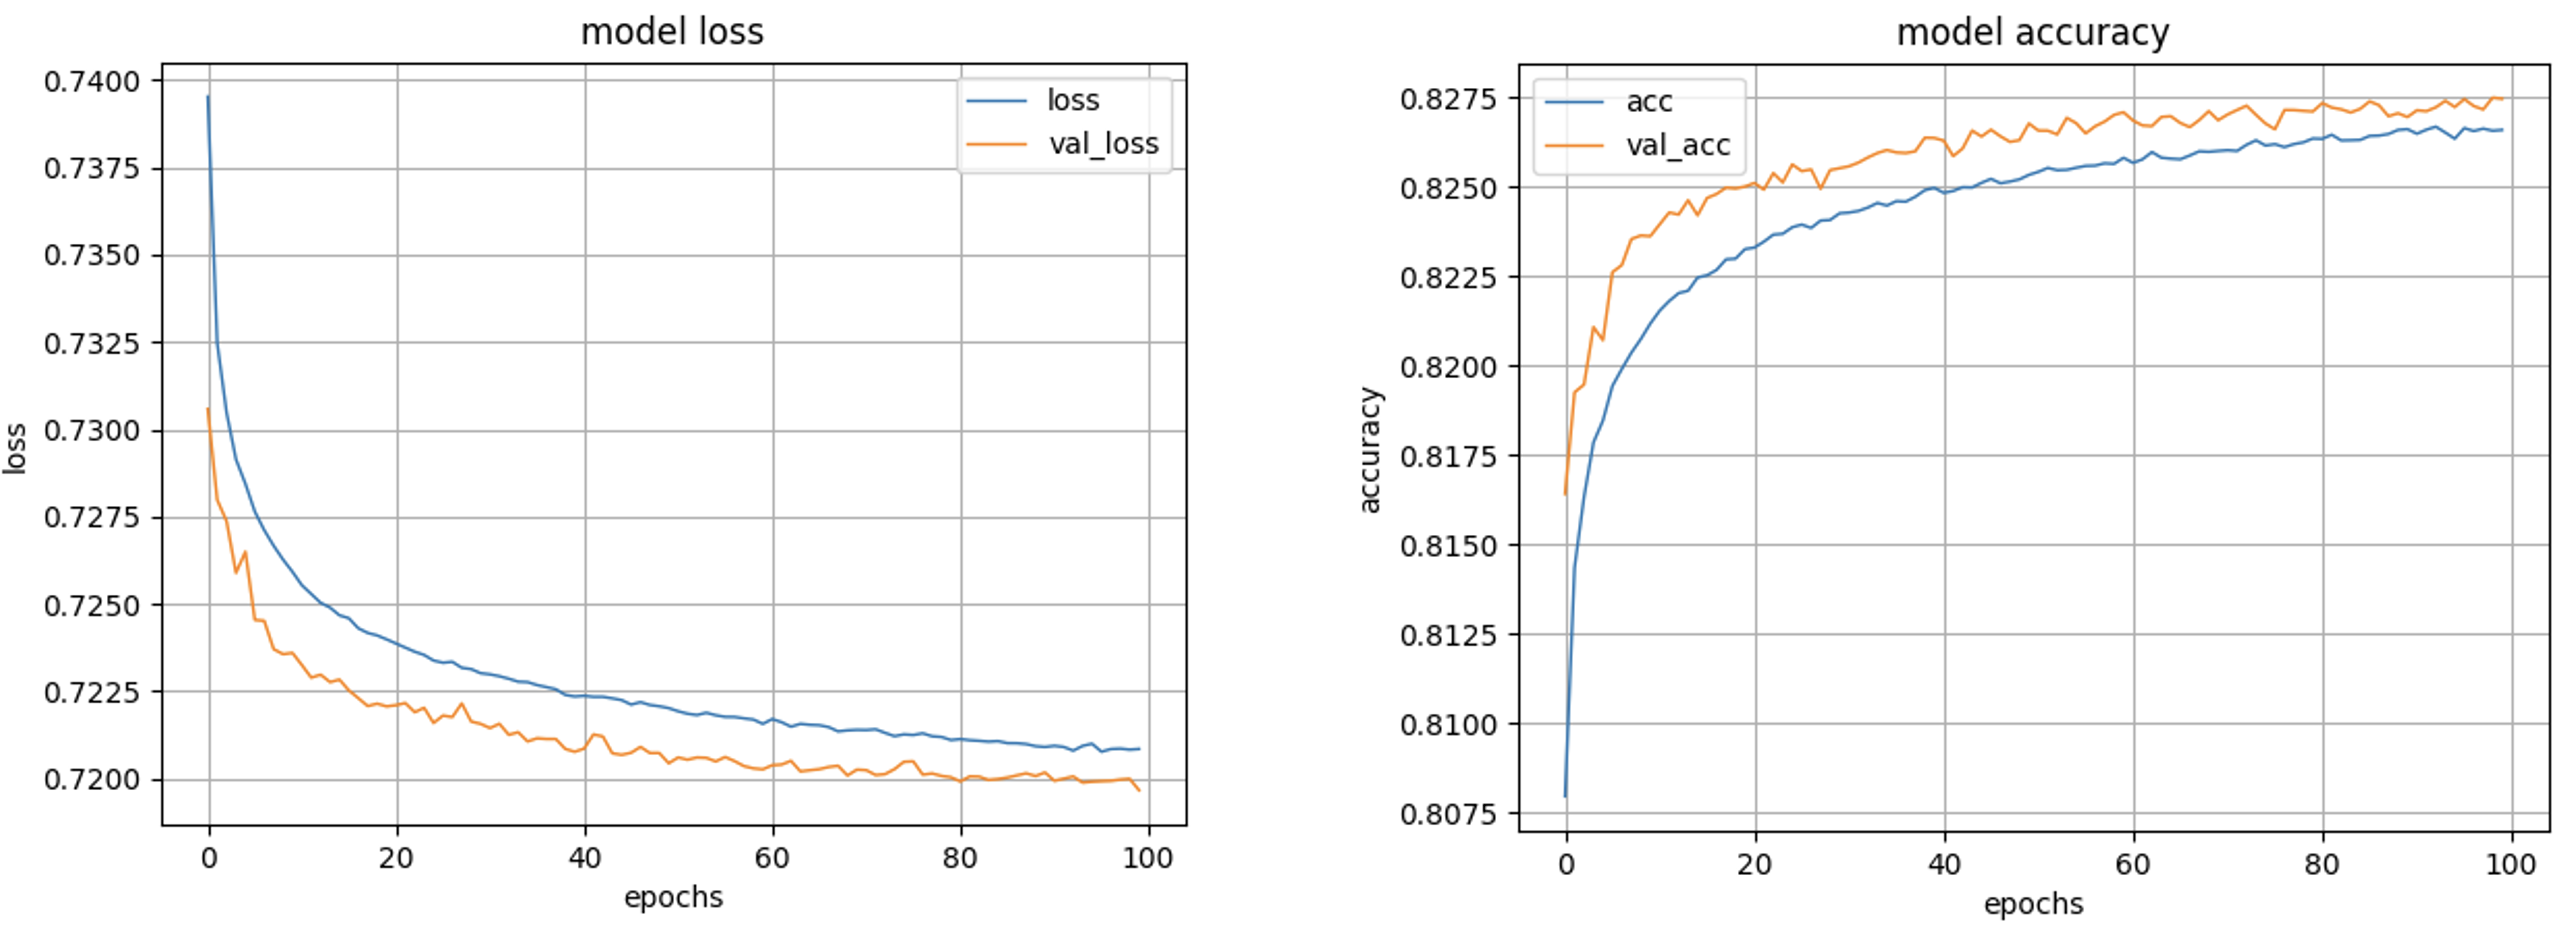
\includegraphics[keepaspectratio, scale=0.3]
 	{Figure/Flavortagging/dnnout.png}
 		\caption{(左)学習の経過における損失関数。(右)学習の経過における学習精度}
 		\label{dnnoutput}
	\end{center}
\end{figure}
\begin{figure}[H]
	\begin{center}
 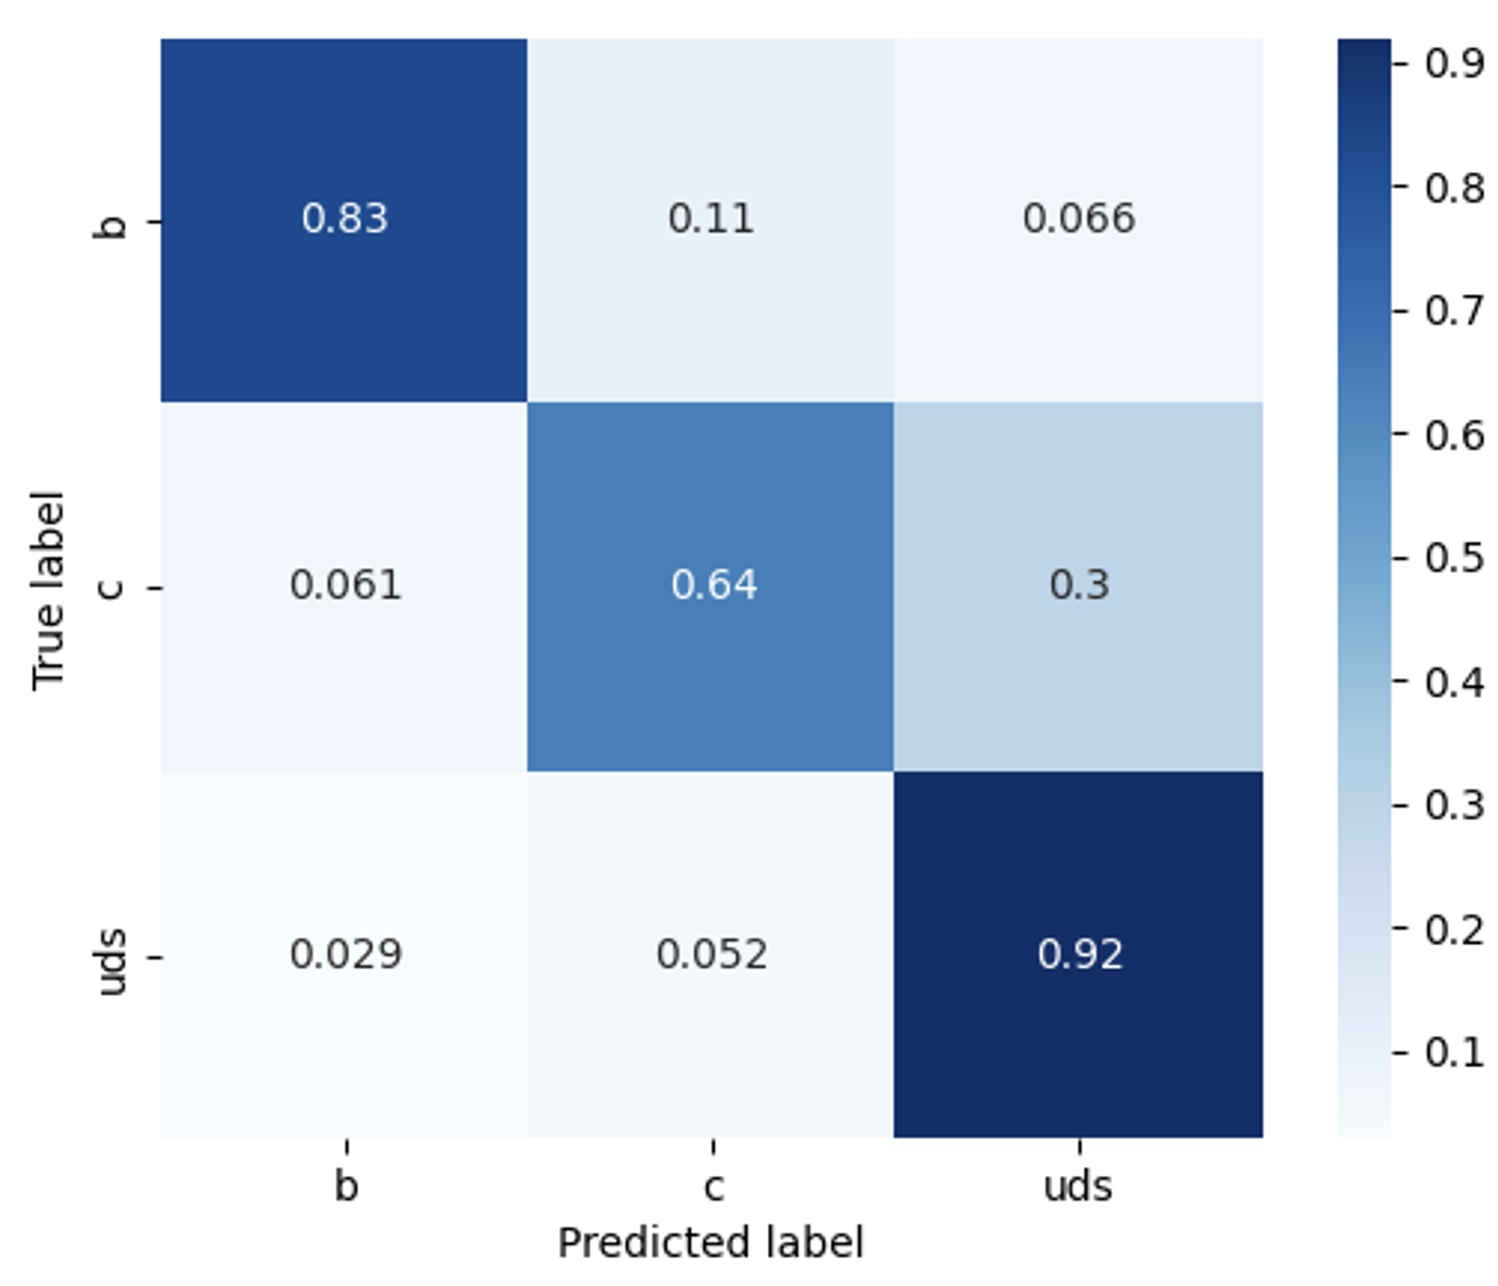
\includegraphics[keepaspectratio, scale=0.2]
 	{Figure/Flavortagging/dnncm.png}
 		\caption{ディープニューラルネットワークの学習における混合行列。縦軸が実際の答えを、横軸が学習結果を表している。}
 		\label{dnncm}
	\end{center}
\end{figure}
次に、LCFIPlusとの比較を示す。本アルゴリズムのモデルの出力値は1つのジェットに対してそれぞれのフレーバーである確率値が得られる。そして、物理解析においてはフレーバー識別の効率が重要であり、識別効率 (= フレーバーをある確率値で決定した場合の正しい認識率) に対して背景事象と誤認識してしまう割合が少なくなることが望ましい。図\ref{dnneff_b}, \ref{dnneff_c}はb/cジェットの識別効率のプロットを、表\ref{dnneff80}は識別効率を$80\%$ (Tagging Efficiency = 0.8) に固定したときの背景ラベルの識別効率の割合を示している。bジェットの識別効率はLCFIPlusと比較して劣っており、特に識別効率$80\%$における識別割合は、LCFIPlusがcジェットの識別割合が$7.3\%$、udsジェットの識別効率が$0.74\%$であるのに対して、ディープニューラルネットのcジェットの識別割合は$20\%程度$、udsジェットの識別効率は$2\%程度$と、udsジェットの識別割合は30倍近く高くなっている。一方でcジェットの識別効率は識別効率$80\%$において、LCFIPlusがbジェットの識別割合が$22\%$、udsジェットの識別効率が$24\%$であるのに対して、ディープニューラルネットのbジェットの識別割合は$数\%程度$、udsジェットの識別効率は$24\%程度$と、bジェットの背景割合は半分以下になっている。本来フレーバー識別はb、cクォークの寿命が長いという特徴を活かして識別するという発想にあるため、崩壊点に関する変数で線形にモデリングしたBDTsでは、cジェットよりもbジェットの方が識別効率が高くなっている。一方でディープニューラルネットワークでは、関係性が逆転している。機械学習アルゴリズムの性能はデータの特性やタスクの種類に大きく依存するため、同じデータを用いていてもアルゴリズムが異なる場合、同じタスクに対する学習特性は異なることがある。今回の場合ではcジェットの識別において、ディープニューラルネットワークでデータ内の複雑な関係を処理できたため、このような結果になったと考えることができる。
\begin{figure}[H]
	\begin{center}
 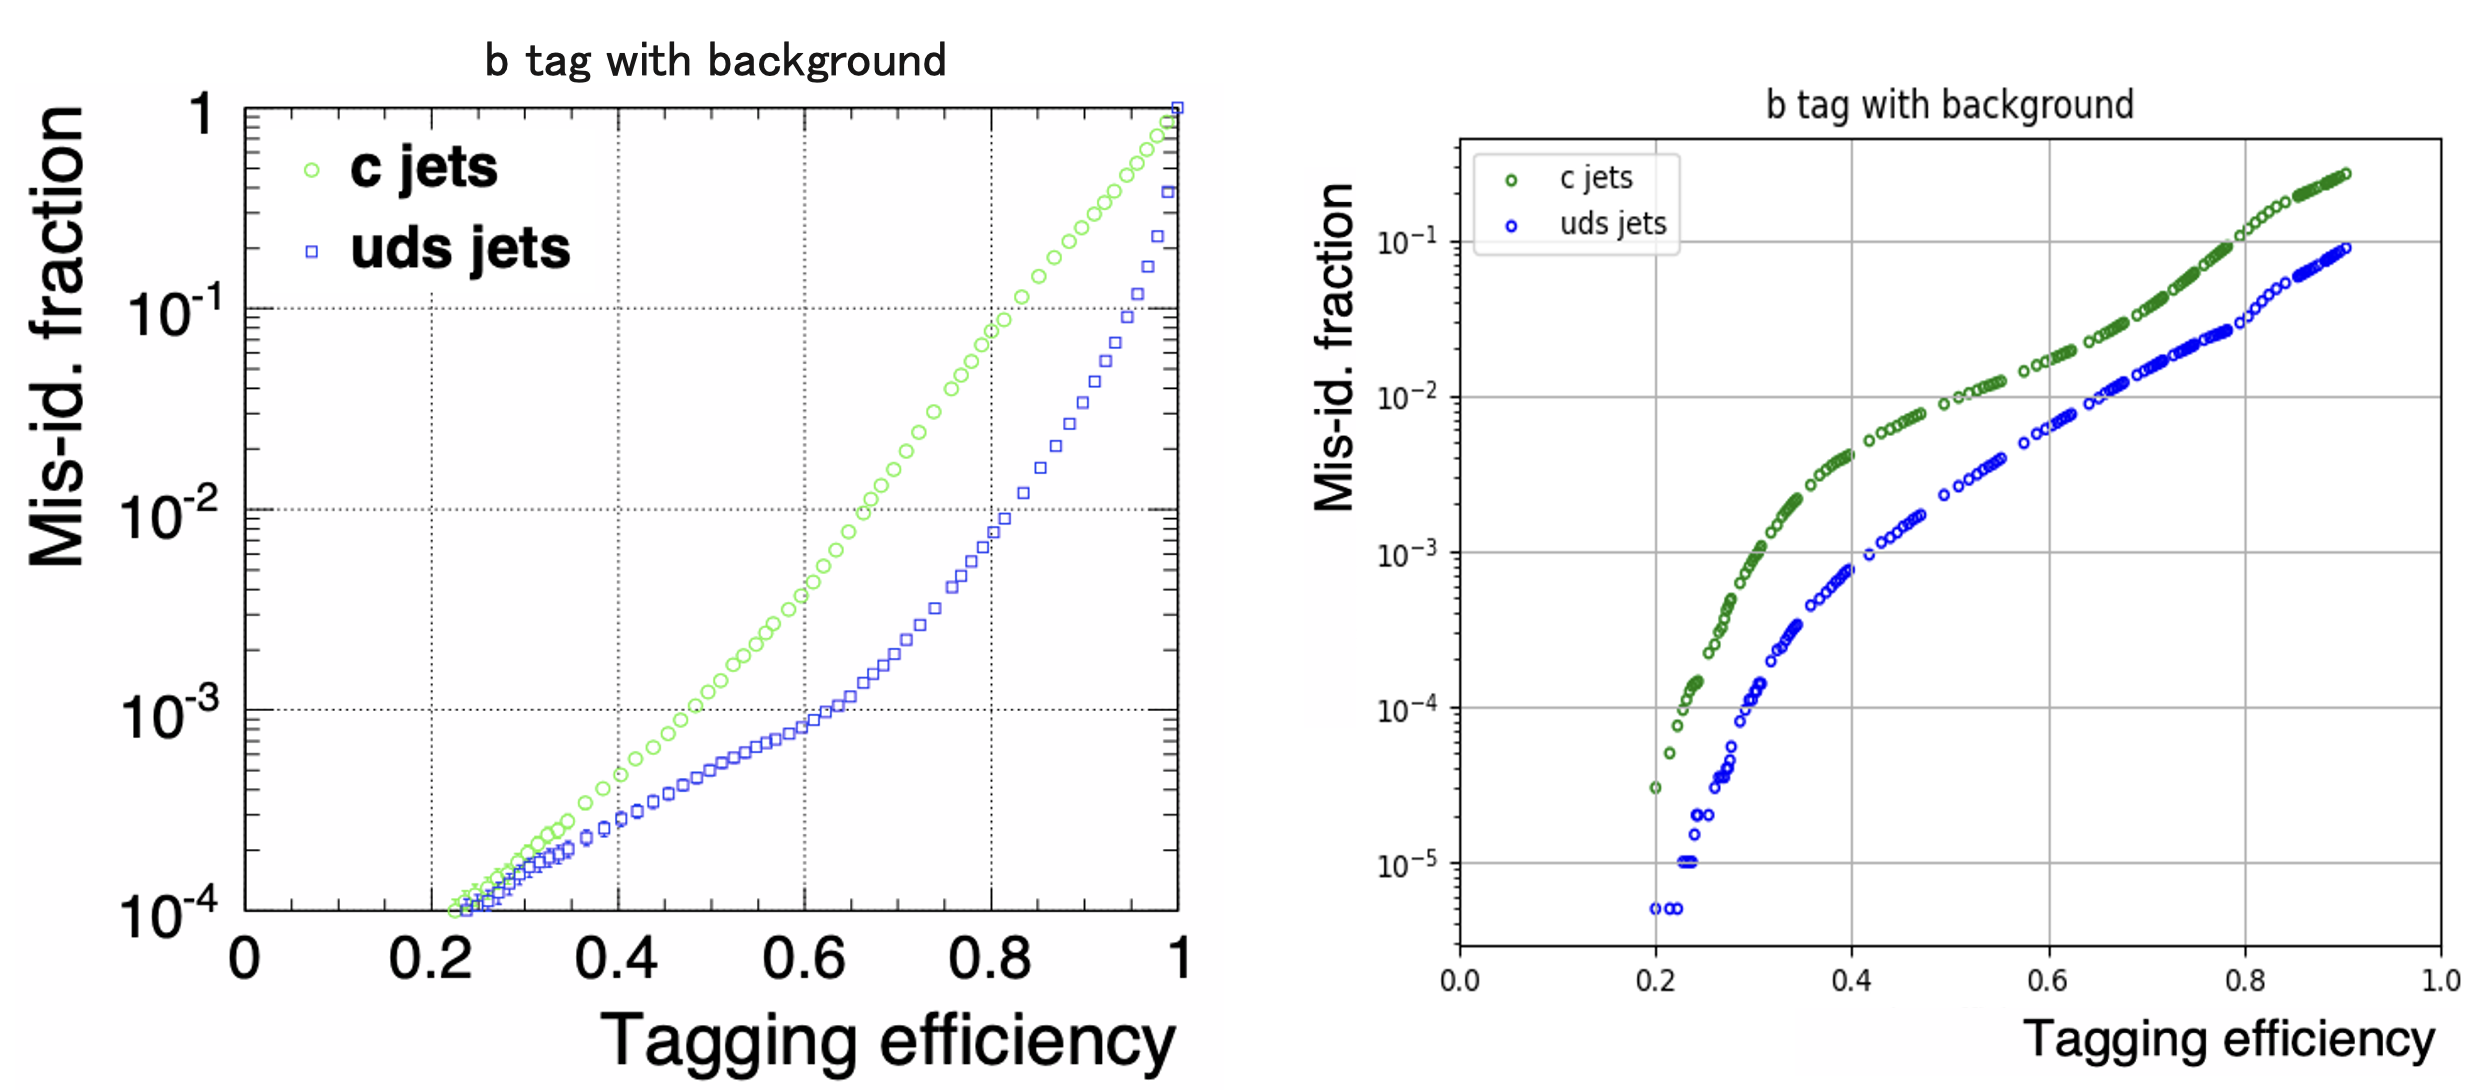
\includegraphics[keepaspectratio, scale=0.3]
 	{Figure/Flavortagging/dnneff_b.png}
 		\caption{LCFIPlus(左)とディープニューラルネットワーク(右)によるbフレーバージェットの識別効率の比較。緑:bジェットに対するcジェットの識別効率、青:bジェットに対するudsジェットの識別効率を示している。}
 		\label{dnneff_b}
	\end{center}
\end{figure}

\begin{figure}[H]
	\begin{center}
 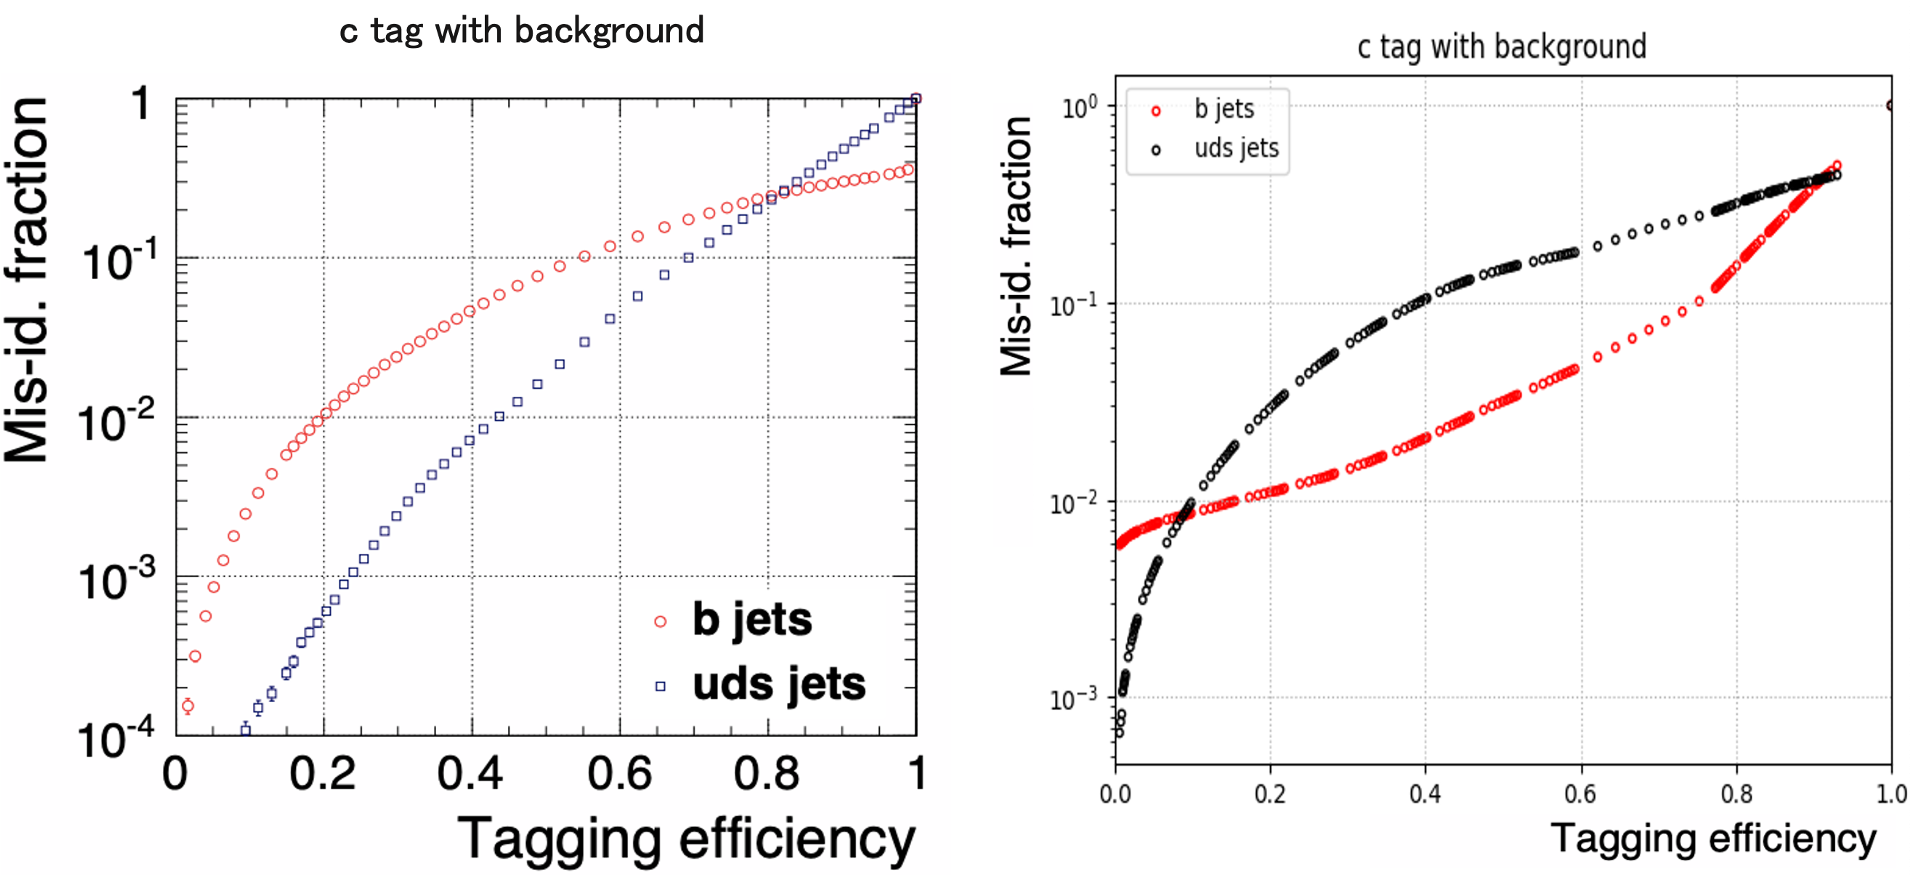
\includegraphics[keepaspectratio, scale=0.3]
 	{Figure/Flavortagging/dnneff_c.png}
 		\caption{LCFIPlus(左)とディープニューラルネットワーク(右)によるcフレーバージェットの識別効率の比較。赤:cジェットに対するbジェットの識別効率、黒:cジェットに対するudsジェットの識別効率。}
 		\label{dnneff_c}
	\end{center}
\end{figure}
\section{グラフニューラルネットワークによる実装}
本節では、グラフニューラルネットワークによるフレーバー識別の実装について述べる。
\subsection{実装目的}
5.3節におけるディープニューラルネットワークの実装では、一部で精度の向上が見られたものの顕著な識別精度の改善はなかった。そこで、ILCのフレーバー識別により最適化した学習を行うために、より高い表現力を持つグラフニューラルネットワークによる実装を考えた。ILCにおけるジェットの物理現象の振る舞いはトポロジカルな構造を持っており、またジェット内の飛跡同士は崩壊点を共有するものが存在している。そのため、グラフデータによってトポロジカルな構造を再現し、データ間の相互関係を活かした学習を行うことで、高い表現力によるアルゴリズムモデルの最適化を目指した。\\
さらにグラフニューラルネットワークの実装では、データをグラフ構造化する上でジェットの内部構造を理解するようなモデルを構築する必要があり、これを補助学習としたアルゴリズムの統合が可能であると考えた。つまり、これまでのようなプロセスを分離した高度なアルゴリズムではなく、1つのアルゴリズム内で飛跡に関する入力変数のみから、飛跡の分類や崩壊点の予想と同時にジェットフレーバーの識別を行うことを可能とするものである。これによって、情報損失を少なくすることで性能の向上を目指すとともに、アルゴリズム調整の単純化や、飛跡の分類結果など将来的に他のアプリケーションに利用可能な情報の生成までもを期待することができる。
\subsection{飛跡によるグラフデータセット}
ILCにおけるジェットの振る舞いを再現するため、本アルゴリズムでは1つのジェットに対して、に飛跡をノードとし全ノードがエッジによって結ばれる1つの同種グラフを構築した。(図\ref{1graph})各ノードは表\ref{gnninput}に挙げる特徴量を入力変数として持ち、エッジは特徴量を持たないものとした。ノードの特徴量には、飛跡に関するパラメータ (Appendix) を用いた。入力データの生成のため、まず250GeVのILDフルシミュレーションにおける$e^+e^- \rightarrow \nu \nu H$事象を使用し、飛跡再構成を行った。続いてLCFIPlusのVertex Fitterプロセスによって、飛跡対が結合する確率値を得た。またシミュレーションにおける答えをもとに3つの学習に対して次のような答えラベルを準備した。それぞれ、ノードの答えラベルは飛跡がどのフレーバージェットのどのvertexから来たものであるのか、エッジの答えラベルは飛跡対が同じ崩壊点を共有するかのバイナリ形式、グラフの答えラベルはどのフレーバーであるのかを答えとした。各学習の答えラベルについて表\ref{gnnoutput_n}$\sim$表\ref{gnnoutput_g}にまとめる。また、入力変数には前処理を行った。さらにデータ数は答えラベル間で偏りがあり、ノードに関するラベルあたりのデータ数\ref{node_imb}はPrimary Vertexを由来とする飛跡が突出して多かったため、比の逆数を重みとして損失関数で考慮することで対応した。
\begin{figure}[H]
	\begin{center}
 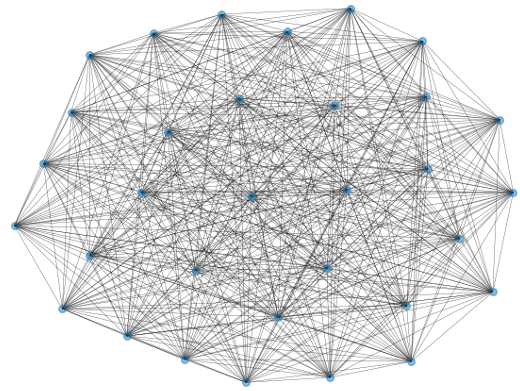
\includegraphics[keepaspectratio, scale=0.5]
 	{Figure/Flavortagging/graphexample.png}
 		\caption{今回の学習に用いたグラフデータの一例。ノードは飛跡を、グラフ全体が1つのジェットに対応する。}
 		\label{1graph}
	\end{center}
\end{figure}

\begin{table}[H]
\centering
 \begin{tabular}{ l  l }
 \hline
 変数名 & 説明\\
 \hline
 \hline
 $d_0$ & xy平面射影におけるIPと飛跡の距離\\
 $\phi$ & xy平面射影における飛跡軌道の方位角\\
 $\omega$ & xy平面射影における飛跡の曲率\\
 $z_0$ & sz平面射影におけるIPと飛跡の距離\\
 $\tan{\lambda}$ &  sz平面射影における$dz/ds$\\
 $\sigma(d_0)$ & $d_0$のフィッティングにおける誤差\\
 $\sigma(z_0)$ & $d_0$のフィッティングにおける誤差\\
 \hline
 \end{tabular}
 \label{gnninput}
 \caption{各ノード (飛跡) が持つ特徴量。詳細についてはAppendixを参照。}
\end{table}

\begin{table}[H]
    \begin{center}
      \begin{tabular}{l l}
         \hline
	ラベル & 説明\\	
	\hline
	\hline
	PV & primary vertex由来の飛跡\\
	SVBB & bフレーバージェットのsecondary vertex由来の飛跡\\
	TVCC & bフレーバージェットのtertiary vertex由来の飛跡\\
	SVCC & cフレーバージェットのsecondary vertex由来の飛跡\\
	Others & 上記の崩壊点を持たない飛跡\\
	\hline
      \end{tabular}
    \end{center}
    \caption{ノード分類の答えラベル}
    \label{gnnoutput_n}
\end{table}
\begin{table}[H]
    \begin{center}
      \begin{tabular}{l l}
         \hline
	ラベル & 説明\\	
	\hline
	\hline
	Connected & エッジの結ぶ飛跡対同士が崩壊点を構成する\\
	Not-Connected & エッジの結ぶ飛跡対同士が崩壊点を構成しない\\
	\hline
      \end{tabular}
    \end{center}
    \caption{リンク予測の答えラベル}
    \label{gnnoutput_e}
\end{table}
\begin{table}[H]
    \begin{center}
      \begin{tabular}{l l}
         \hline
	ラベル & 説明\\	
	\hline
	\hline
	$b\bar{b}$ & bフレーバージェット\\
	$c\bar{c}$ & cフレーバージェット\\
	$q\bar{q}$ & udsフレーバージェット\\
	\hline
      \end{tabular}
    \end{center}
    \caption{グラフ分類の答えラベル}
  \label{gnnoutput_g}
\end{table}
\begin{figure}[H]
	\begin{center}
 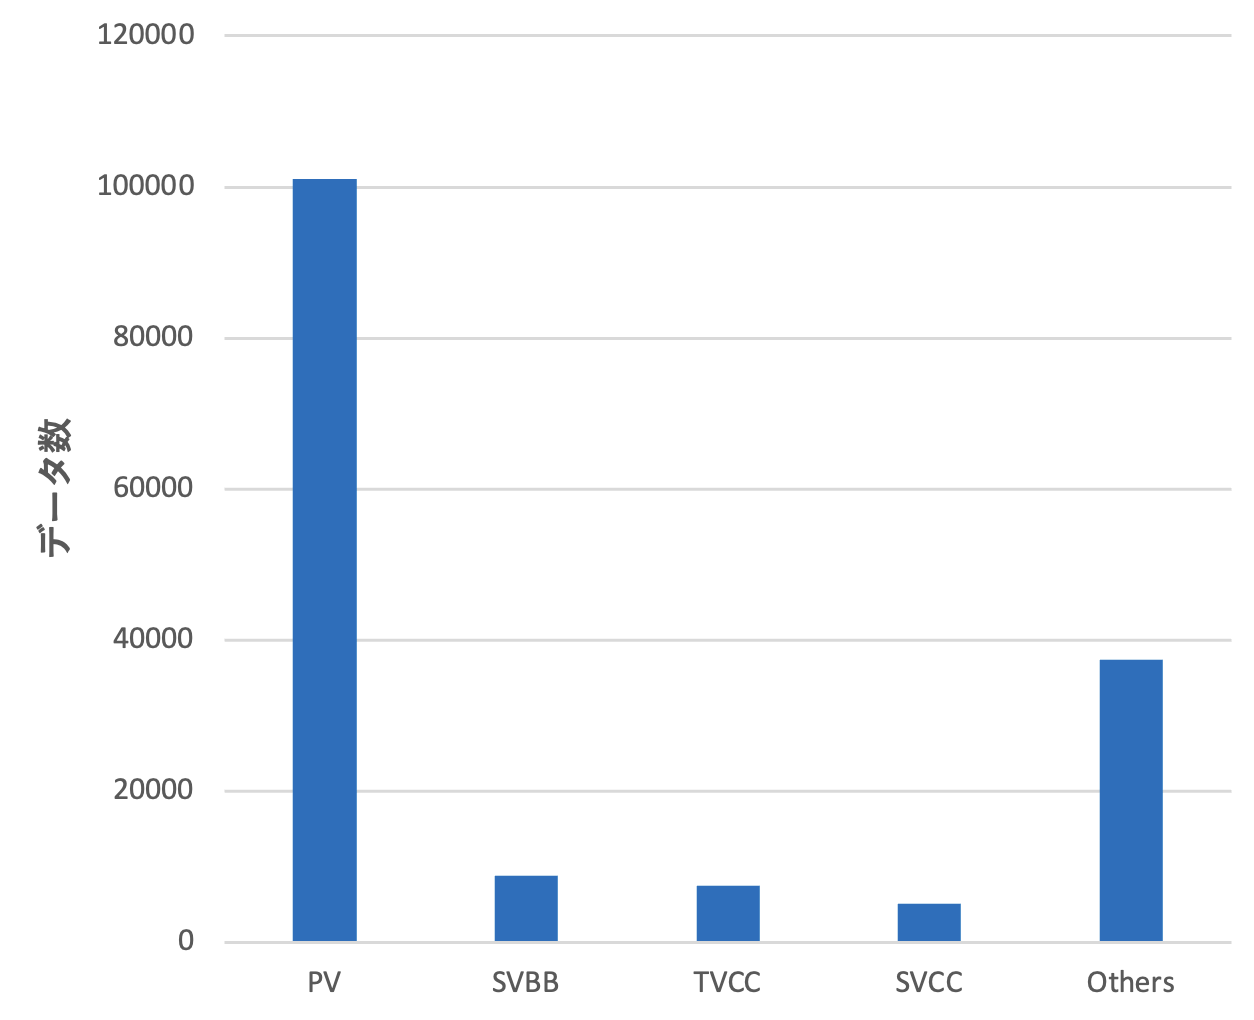
\includegraphics[keepaspectratio, scale=0.5]
 	{Figure/Flavortagging/imbalance.png}
 		\caption{ノードラベル毎のデータ数}
 		\label{node_imb}
	\end{center}
\end{figure}
\subsection{ネットワークアーキテクチャ}
上述の通り、本アルゴリズムではフレーバー識別に加えて、補助学習を導入する。具体的にはノード分類とリンク予測、グラフ分類の3つのタスクを同時に行うネットワークで、図\ref{gnnmodel}のようなモデルを構築した。\\
はじめに、飛跡の変数をより多次元ベクトル化し潜在表現を得るために全結合層を設置する。その後、Graph Attention Network (GAT) を3層設置し、各GAT層の後にはバッチ正規化とReLU関数の活性化関数を置く。そして学習をノード分類、リンク予測、グラフ分類の3つに分岐させる。ノード分類では、飛跡の由来となる崩壊点の種類によって5つの出力が全結合層によって設計されている。リンク予測では、エッジの隣接行列を取得してノード間に隣接があるかないかを判断する2分類問題を行っており、これはエッジが崩壊点となりうるのかの判断に等しい。グラフ分類では、poolingによってグラフ全体の特徴量を1つの次元に置き換え、各フレーバーらしさを出力する設計になっている。\\
GATの学習は\ref{GATexplain}節で述べた通りであり、本アルゴリズムのグラフデータは全結合のグラフニューラルネットワークを構築しており、ノードに対するアテンション$\alpha$はエッジの隣接関係を用いて式\ref{gatattention}のように学習される。このようなアテンション機構によってグラフ全体、すなわちジェットフレーバーの識別を補助することを目的に、ノードの識別の補助学習を導入した。また、実際に飛跡対が崩壊点を共有している場合、その隣接関係は物理的に重要なものとなるため、その情報を学習に活かすことを目的にリンク予測を補助学習に加えた。また、3つの学習の出力層に置いた全結合層はそれぞれ独立に実行される。\\
\begin{figure}[H]
	\begin{center}
 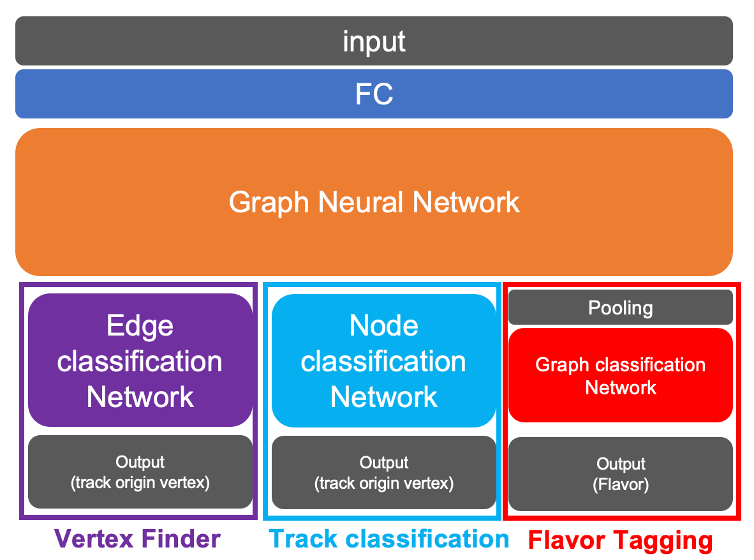
\includegraphics[keepaspectratio, scale=0.4]
 	{Figure/Flavortagging/gnn.png}
 		\caption{フレーバー識別のためのグラフデータを用いたネットワークの概略図}
 		\label{gnnmodel}
	\end{center}
\end{figure}
また本アルゴリズムでは3つの異なる学習を同時に行う必要があり、目的によって相対的な学習のしやすさが異なるため、次のような損失関数をデザインした。\\
\begin{align}
\mathrm{L}_{total} = \mathrm{L}_{graph} + w_{node} \mathrm{L}_{node} + w_{edge} \mathrm{L}_{edge}
\end{align}
$\mathrm{L}$はそれぞれの損失関数を、$w_{node}とw_{edge}$はそれぞれノード、エッジの損失関数にかける重みを表す。グラフ識別と同程度の損失関数に収束するために、ノード識別とリンク予測における損失関数に重み付けを行った。\\
\ また、学習におけるハイパーパラメータにはベイズ最適化を行った上で、表\ref{gnnsetting}に挙げるものを用いた。
\begin{table}[H]
 \centering
  \begin{tabular}{ l  l }
   \hline
   ノード数 & (512, 512, 512)\\
   活性化関数 & ReLU関数\\
   損失関数 & 交差エントロピー\\
   最適化アルゴリズム & RAdam\\
   学習率 & 0.01\\
   Weight decay & 0.0001\\
    $w_{node}$ & 3.0\\
    $w_{edge}$ & 1.0\\
   エポック数 & 100\\
   バッチサイズ & 128\\
   \hline
  \end{tabular}
  \label{gnnsetting}
  \caption{グラフニューラルネットワークにおけるハイパーパラメータ}
\end{table}
\subsection{ハイパーパラメータの最適化}
ネットワークのハイパーパラメータは、ベイズ最適化法によってチューニングを行った。チューニングしたパラメータは表\ref{gnnoptuna}を用いた。チューニングにはディープニューラルネットワークの実装におけるものと同じライブラリを用いたが、評価関数として検証用データの損失関数のうち$ \mathrm{L}_{graph}$のみを用いて、最小になるような最適化を行った。
\begin{table}[H]
\centering
 \begin{tabular}{ l  l }
 \hline
 変数名 & 最適化範囲\\
 \hline
 \hline
 中間層のノード数 & $32 \sim 1024$\\
 アテンションヘッドの数 & $1 \sim 20$\\
 $\alpha$ & $0.0 \sim 5.0$\\
 $\beta$ & $0.0 \sim 5.0$\\
  \hline
 \end{tabular}
 \label{gnnoptuna}
 \caption{最適化を行ったハイパーパラメータとその値の範囲。}
\end{table}
\subsection{学習評価}
はじめに、学習全体の結果を図\ref{gnnoutput}に示す。学習の経過を通して損失関数は減少しており、特に80epoch付近で急激な降下を見せた。しかしそれ以降は過学習が進んでしまい、損失関数の値は安定化させることが難しかった。また、ノード、リンク、グラフそれぞれの精度においても、学習の経過を通して向上が見られた。\\
\begin{figure}[H]
	\begin{center}
 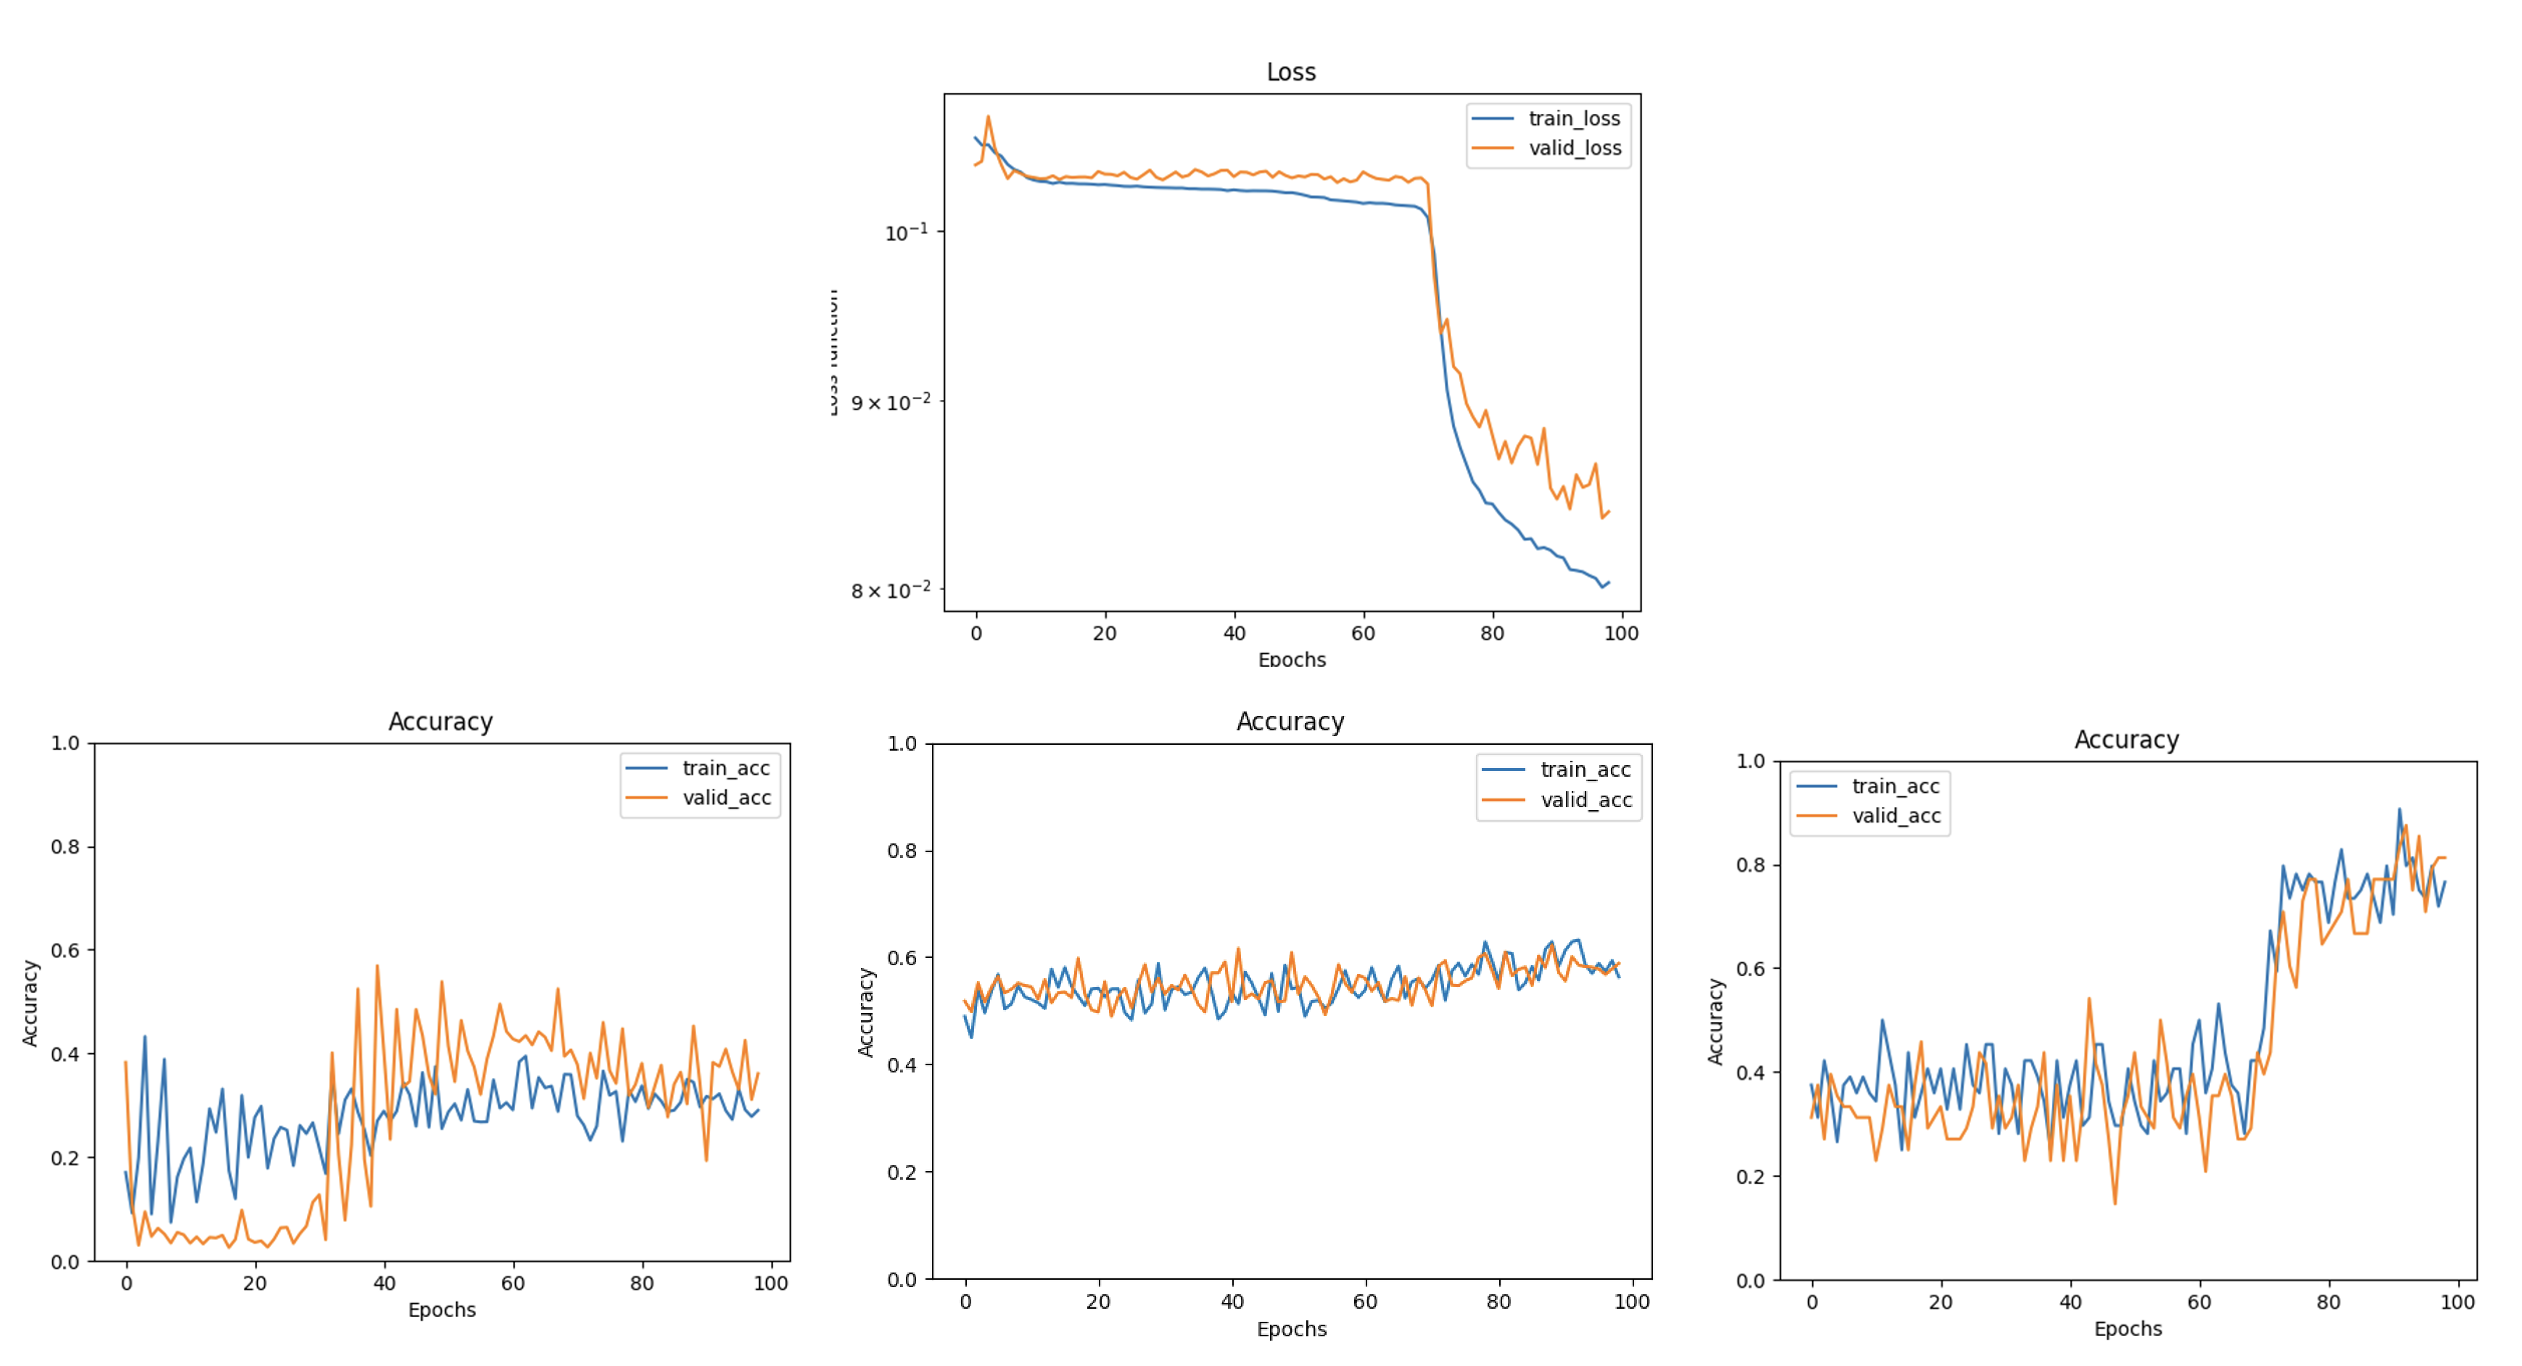
\includegraphics[keepaspectratio, scale=0.3]
 	{Figure/Flavortagging/gnnoutput.png}
 		\caption{(上)学習の経過における損失関数。(左下) 学習の経過におけるノードの学習精度、(中央下) リンクの学習精度、(右下) グラフの学習精度。}
 		\label{gnnoutput}
	\end{center}
\end{figure}
続いて、ノード、リンク、グラフ識別における混合行列を図\ref{gnncm}に示す。ノード、リンクの学習精度は十分良いと言える制度ではなく、一方でグラフの識別においてはディープニューラルネットワークでの実装に匹敵する精度が得られた。ノードの混合行列ではPVとSVBBと識別する割合が高く、一方でTVCC、Othersについて分類が出来ずPVに分類されてしまう傾向にあった。\\
\begin{figure}[H]
	\begin{center}
 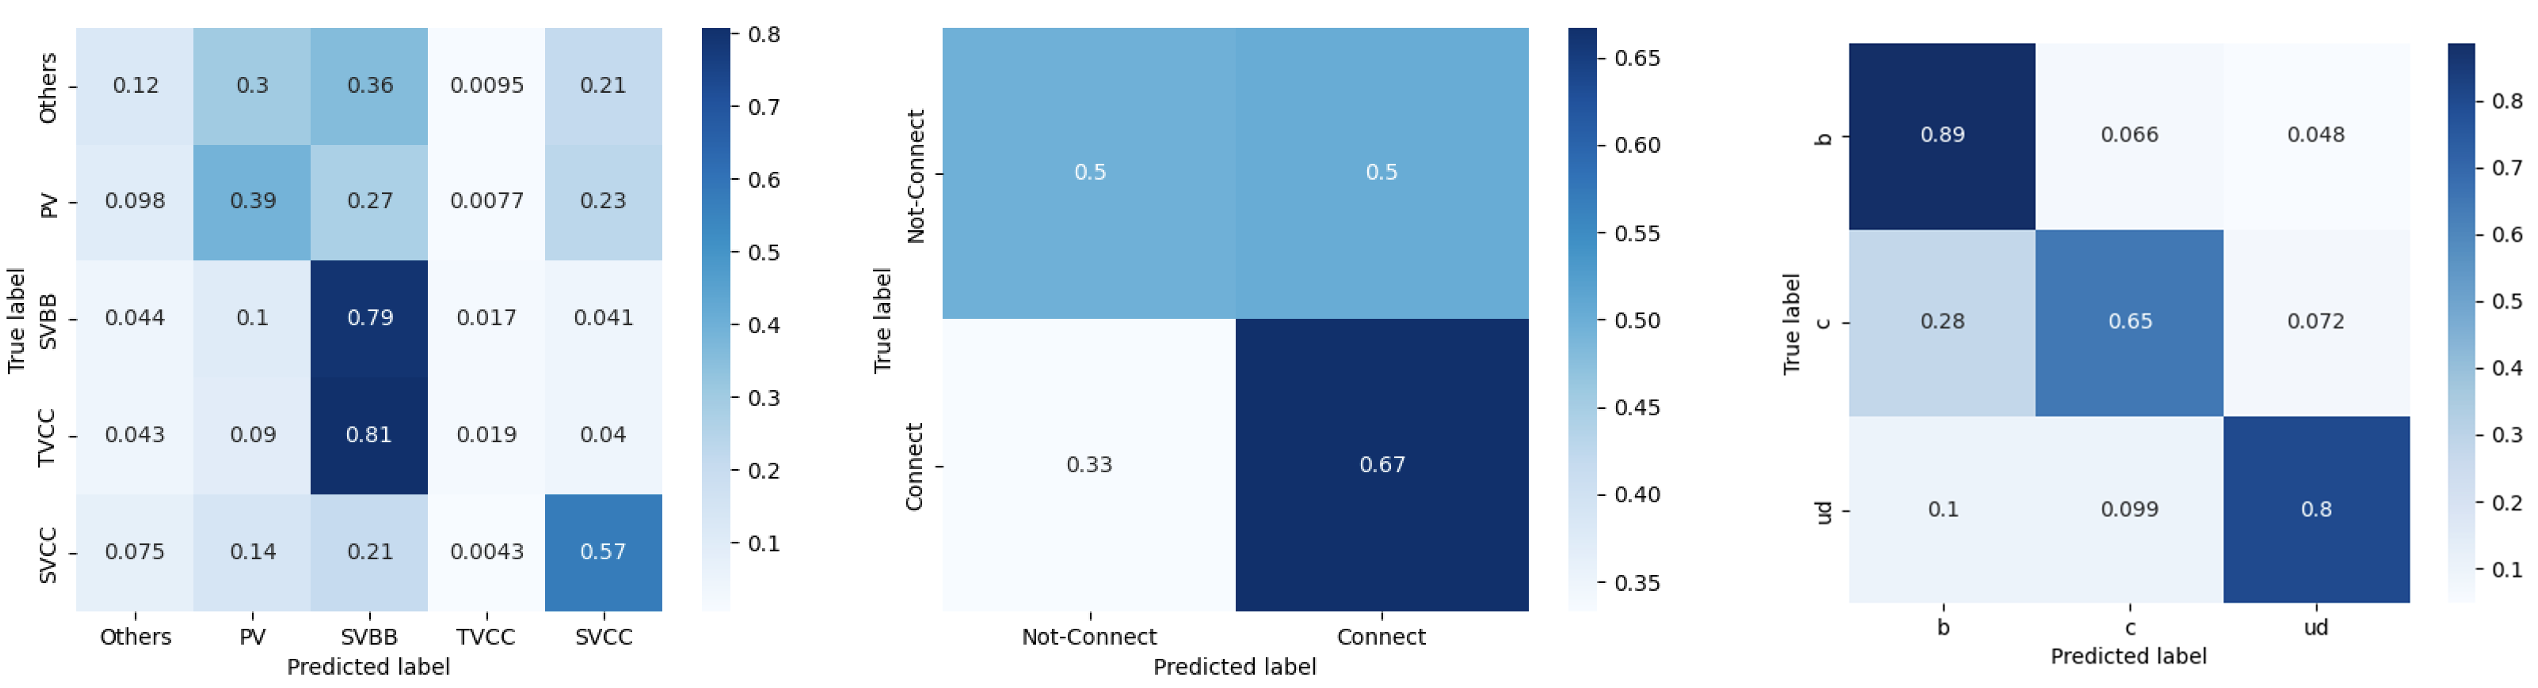
\includegraphics[keepaspectratio, scale=0.3]
 	{Figure/Flavortagging/gnncm.png}
 		\caption{(左) ノード分類の混合行列、(中央) リンク予測の混合行列、(右) グラフ識別の混合行列。}
 		\label{gnncm}
	\end{center}
\end{figure}
最後に、LCFIPlusとの比較を示す。ディープニューラルネットワークの比較と同様に、図\ref{gnneff_b}, \ref{gnneff_c} は b/c ジェットの識別効率のプロットを、表\ref{gnn_lcfi}は識別効率を 80\% (Tagging Efficiency = 0.8) に固定したときの背景ラベルの識別効率の 割合を示している。bジェットの識別効率はcジェットについて向上しており、識別効率80\%における識別割合は、LCFIPlus が c ジェットの識別割合が 7.3\%、uds ジェットの識別効率が 0.74\% であるのに対して、グラフニューラルネットワークのcジェットの識別割合はおよそ1.5\%、udfジェットの識別効率もおよそ1\%ほどという結果になり、cジェットの誤認率が5分の1程度になっているものの、udsジェットに関しては若干の精度低下となった。また、cジェットの識別効率は非常に悪い結果となってしまい、識別効率80\%における識別割合は、LCFIPlus がbジェットの識別割合が 22\%、udsジェットの識別効率が 24\% であるのに対して、グラフニューラルネットワークのbジェットの識別割合はおよそ40\%、udfジェットの識別効率はおよそ15\%ほどという結果になり、bジェットの誤認率が2倍近く上がってしまった。ノード分類結果では、PVとSVBBと識別する割合が高いことから、bジェットに対する識別効率が高くなっていることが考えられる。また、cジェットのbジェットとの分離が悪い点に関しては、主にSVBB,TVCCに対するSVCCの分類精度が課題となっていると推測される。\\
\begin{figure}[H]
	\begin{center}
 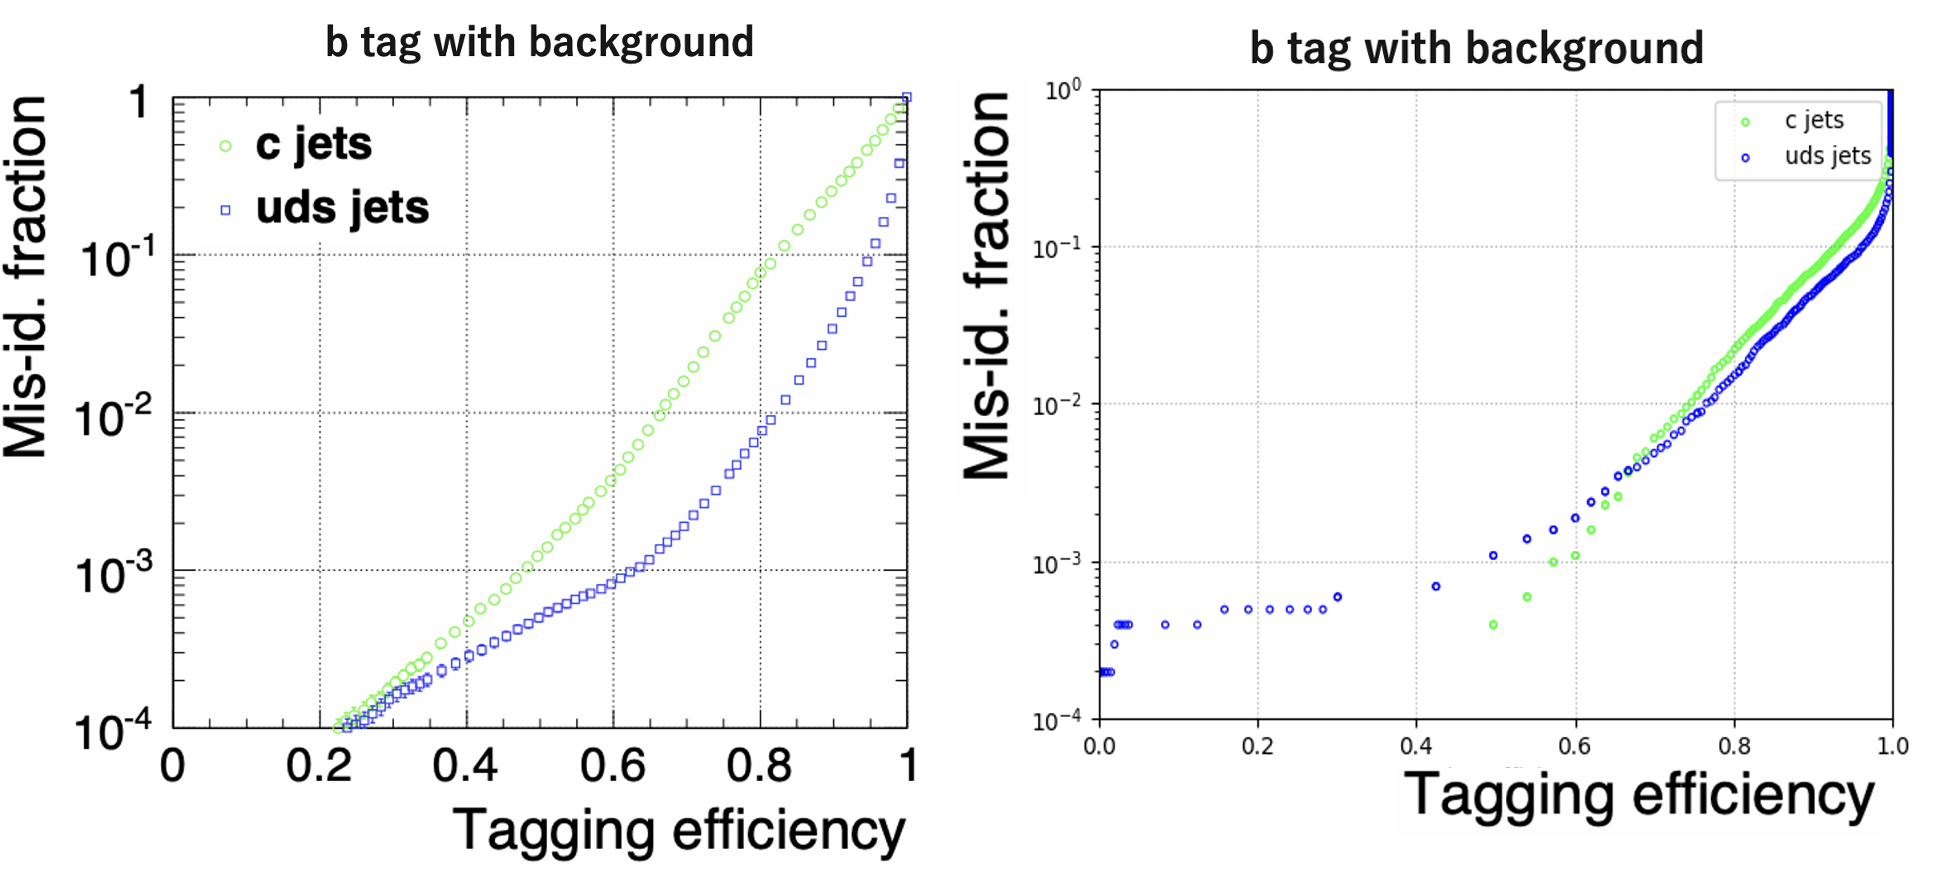
\includegraphics[keepaspectratio, scale=0.3]
 	{Figure/Flavortagging/gnneff_b.png}
 		\caption{LCFIPlus(左)とグラフニューラルネットワーク(右)によるbフレーバージェットの識別効率の比較。緑:bジェットに対するcジェットの識別効率、青:bジェットに対するudsジェットの識別効率を示している。}
 		\label{gnneff_b}
	\end{center}
\end{figure}

\begin{figure}[H]
	\begin{center}
 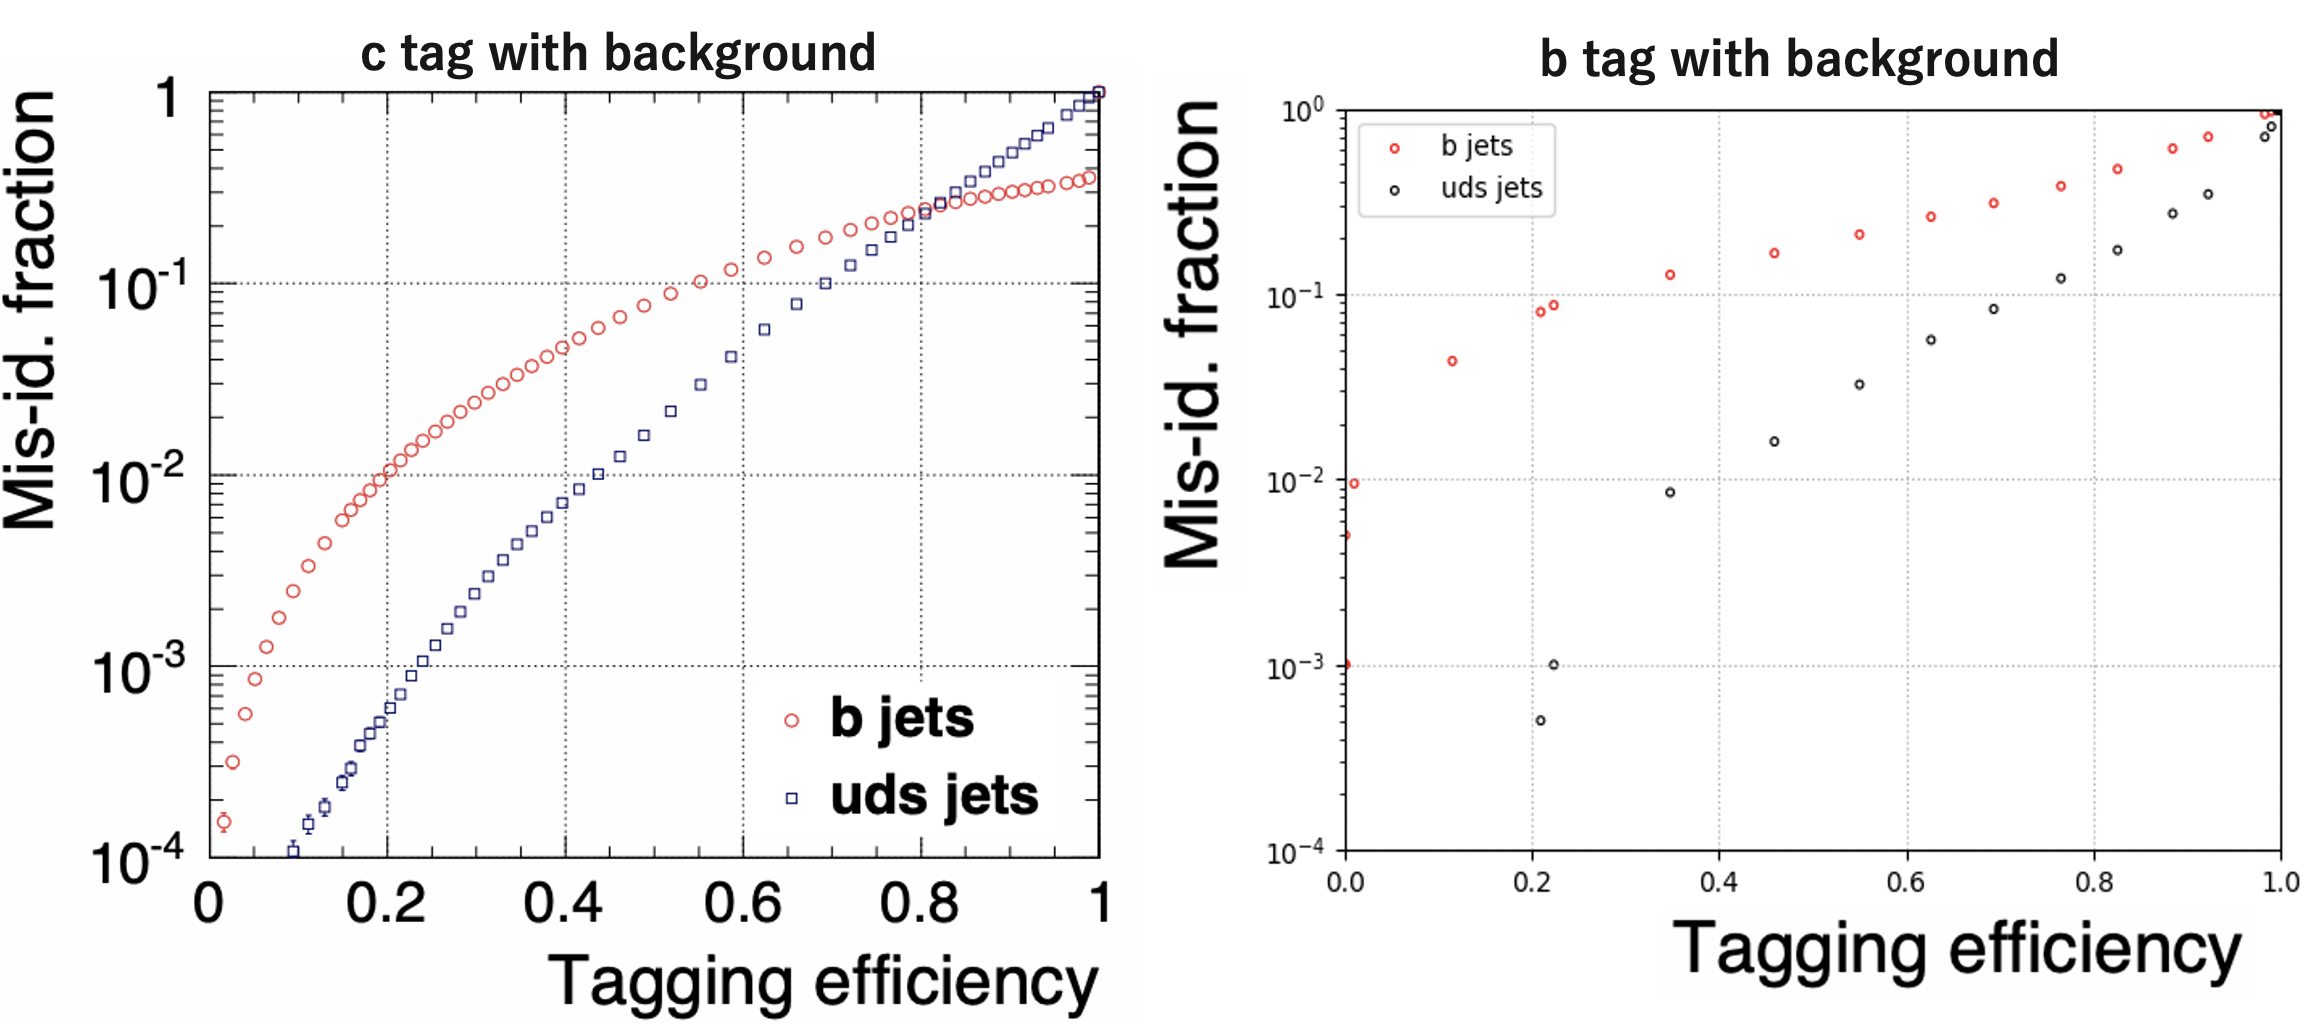
\includegraphics[keepaspectratio, scale=0.3]
 	{Figure/Flavortagging/gnneff_c.png}
 		\caption{LCFIPlus(左)とグラフニューラルネットワーク(右)によるcフレーバージェットの識別効率の比較。赤:cジェットに対するbジェットの識別効率、黒:cジェットに対するudsジェットの識別効率。}
 		\label{gnneff_c}
	\end{center}
\end{figure}
結果として、グラフニューラルネットワークによる実装ではLCFIPlusと比較して顕著な性能向上があったとは言えない結果になった。しかしながらエッジリンク予測の実行によって、これまで別のプロセスで実行していた崩壊点検出を、1つのネットワーク内で内包することが出来た。